\subsection{General}

Desarrollar un sistema basado en Deep Learning que permita localizar zonas activas cerebrales a partir de señales EEG preprocesadas, mediante un modelo inverso.

\subsection{Específicos}
\begin{enumerate}
    \item \textbf{Generación y Preprocesamiento de Señales EEG}

    Generar señales electroencefalográficas (EEG) artificiales correspondientes a la actividad cerebral relacionada con la activación de grupos musculares. Identificando segmentos de señal válidos que puedan ser utilizados para el análisis posterior.

    \item \textbf{Diseño y Entrenamiento del Modelo Inverso}

    Desarrollar un modelo inverso capaz de estimar la localización tridimensional de las fuentes neuronales responsables de las señales EEG registradas en la superficie del cuero cabelludo utilizando redes neuronales profundas. El desempeño del modelo será evaluado mediante pruebas controladas, incluyendo simulaciones con fuentes conocidas y validación cruzada con registros reales.

    \item \textbf{Identificación de Zonas de Activación Cerebral}

    Determinar las regiones corticales activas asociadas con la ejecución de tareas motoras específicas, comparando la localización estimada por el modelo con datos anatómicos y funcionales disponibles. 

    \item \textbf{Verificación la efectividad del modelo}

    Verificar la efectividad del modelo propuesto mediante métricas cuantitativas aplicadas a datos simulados y reales. Comparar datos de modelos existentes en igualdad de condiciones.
\end{enumerate}

\subsection{Cronograma}
\begin{landscape}
\begin{figure}%[H]
    \centering
    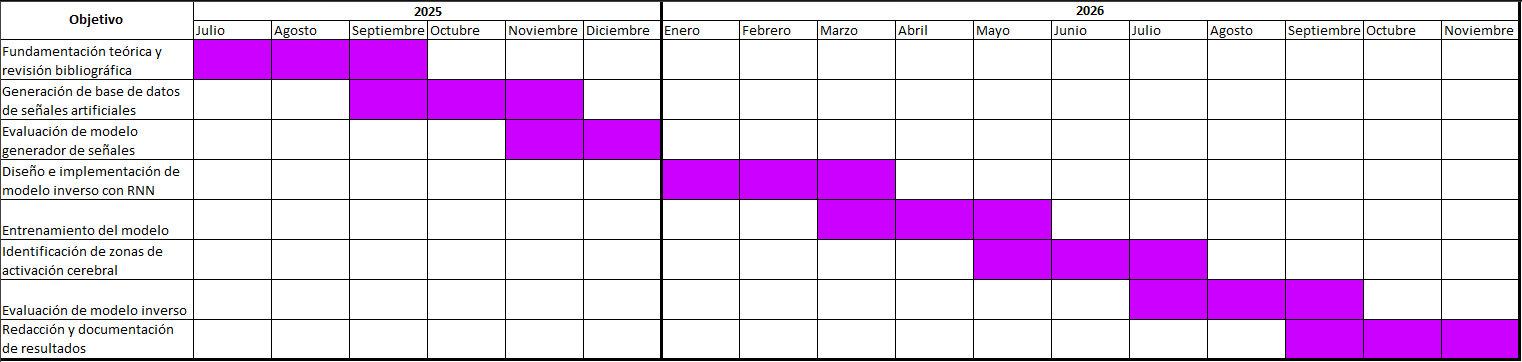
\includegraphics[scale=0.4]{figures/obj/cronograma.png}
    \caption{Cronograma de Actividades}
    \label{fig:crono}
\end{figure}
\end{landscape}